\section{The Birth of Software Engineering}

\subsection{Development of Hardware/Software and Their Relationship}

\begin{itemize} \item \textbf{\underline{1940-1950: Vacuum Tubes}}:
Vacuum tubes were electronic components that controlled the flow of electricity in a vacuum. Used in radios, televisions, and early computers, they were large, expensive, and consumed a lot of power, but were essential for electronics at the time.



\item \textbf{\underline{1950-1960: Transistors}}:  
Transistors are semiconductor devices used to amplify or switch electronic signals. They replaced vacuum tubes due to their smaller size, greater efficiency, and lower cost. Transistors were used in radios, early computers, and have since become fundamental in all modern electronics.

\item \textbf{\underline{1960-1970: Integrated Circuits}}:  
An integrated circuit (IC) is a small chip that contains a set of electronic circuits, including transistors, resistors, and capacitors. ICs made electronics more compact, affordable, and powerful, revolutionizing industries during the 1960s. ICs were found in computers, calculators, and a wide range of other electronic devices.

\item \textbf{\underline{1970-Present: Microprocessors}}:  
A microprocessor is a single-chip CPU (Central Processing Unit) that performs the functions of a computer's central processor. Microprocessors became more affordable in the 1970s, paving the way for the rise of personal computers, smartphones, and embedded systems in countless devices today.

\end{itemize}

\vspace{0.5cm}
\begin{center}
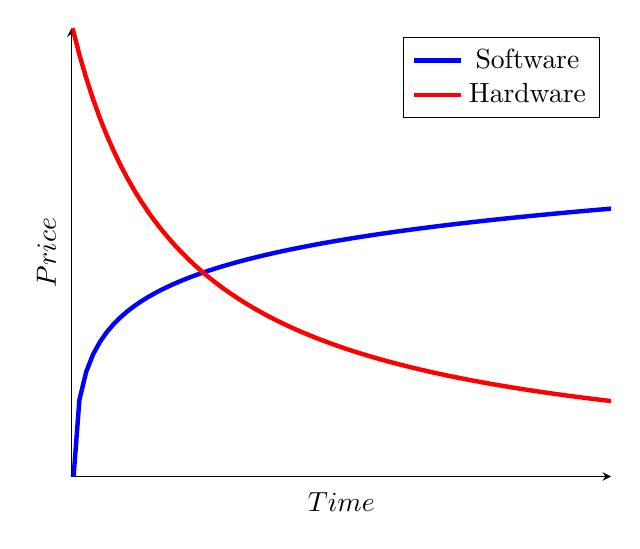
\begin{tikzpicture} 
\begin{axis}[ axis lines = left,
              xlabel=$Time$, 
              ylabel=$Price$, 
              domain=0.01:5, 
              xtick=\empty, 
              ytick=\empty, 
              xmin=0,
              ymin=0] 
\addplot[ultra thick, color = blue, no marks, samples = 80] {5 + ln(0.5*x)}; 
\addlegendentry{Software} 
\addplot[ultra thick, color = red, no marks, samples = 80] {10 / (x + 1)}; 
\addlegendentry{Hardware} 
\end{axis} 
\end{tikzpicture}
\end{center}
\vspace{1.5cm}

As shown in the graph above, there is an inverse relationship between hardware and software prices. As hardware becomes more affordable and advanced, software prices tend to increase, a phenomenon often referred to as the "Software Crisis." This was primarily caused by a lack of development methodology and reflection on part of the developers. Software projects frequently went over budget, were late to release, and were often filled with bugs.

To address this issue, developers needed to establish efficient methodologies and practices for building better software.

\subsection{Qualities of Good Software}


A well-designed software product must meet several key criteria to be considered high-quality. Here are some essential qualities:

\begin{itemize}

\item \textbf{Maintainability}:
The ease with which software can be modified to correct faults, improve performance, or adapt to a changed environment. Code should be well-documented, modular, and easy to update without causing regressions in other parts of the software.


\item \textbf{Affordability}:  
High-quality software should provide value for money. The cost of development, licensing, maintenance, and support should be reasonable and aligned with the customer's budget and expectations. Affordability doesn't mean the cheapest option, but one that balances cost with features and reliability.

\item \textbf{Functionality}:  
The software must meet the specific needs of its users and perform the tasks it was designed for effectively. It should deliver all required features and capabilities, ensuring that it fulfills its purpose.

\item \textbf{Reliability}:  
Software should function consistently and accurately over time, without crashing or producing incorrect results. It should handle errors gracefully and work well under various conditions, including edge cases and unexpected inputs.

\item \textbf{Performance}:  
Good software should operate efficiently, with fast response times and minimal use of system resources. Performance includes aspects like load times, memory usage, and the ability to handle multiple tasks or large amounts of data simultaneously.

\item \textbf{Scalability}:  
The software should be able to grow and accommodate increasing amounts of work or users without a significant drop in performance. This is especially important for systems that expect long-term growth or fluctuating demand.

\item \textbf{Usability}:  
The user interface should be intuitive, making it easy for users to learn and navigate. Well-designed software provides a positive user experience, with thoughtful layouts, clear instructions, and accessible features for all users, including those with disabilities.

\item \textbf{Security}:  
Security is critical in today's environment. High-quality software should protect user data and prevent unauthorized access, ensuring compliance with security standards. It should include features like encryption, authentication, and protection against common vulnerabilities such as SQL injection or cross-site scripting.

\item \textbf{Portability}:  
Software should work across different platforms and environments with minimal modifications. This is especially important for applications intended to run on multiple operating systems, browsers, or devices. A portable software solution can save significant development effort.

\item \textbf{Interoperability}:  
High-quality software should be able to integrate and work seamlessly with other systems and tools. This includes support for standard formats, APIs, and protocols that allow it to exchange data and collaborate with other software.

\item \textbf{Minimization of Bugs}:  
A good software product should have a minimal number of defects. This involves rigorous testing during the development process to catch and fix bugs early, as well as ongoing maintenance and updates to address issues as they arise.

\item \textbf{Extensibility}:  
Software should be designed in a way that allows new features and functionality to be added in the future without significant changes to the core architecture. Extensible software can adapt to changing user needs and technology advances.

\item \textbf{Compliance with Standards}:  
High-quality software adheres to industry standards and regulations, ensuring that it meets legal, technical, and ethical guidelines. This is particularly important in industries like healthcare, finance, and government, where compliance is mandatory.
\end{itemize}

\vspace{0.5cm}
\begin{center}
\begin{tikzpicture} 
\begin{axis}[ axis lines = left,
              xlabel=$Quality$,
              ylabel=$Price$,
              domain=0.01:5,
              xtick=\empty,
              ytick=\empty,
              xmin=0, 
              ymin=0] 
\addplot[ultra thick, color = blue, no marks, samples = 80] {exp(x)}; 
\end{axis} 
\end{tikzpicture}
\end{center}
This graph illustrates the positive correlation between software quality and price. As the quality of the software improves, its price tends to increase exponentially.
